\documentclass[10pt]{article}
\usepackage{fontspec,luatexja-fontspec}
\setmainjfont{HaranoAjiMincho-Regular.otf}
\usepackage[letterpaper,margin=.9in]{geometry}
\usepackage{amsmath,amssymb,graphicx,caption,booktabs,float,hyperref}
\captionsetup{font=small,labelfont=bf}
\newcommand{\Cris}{\mathcal C}\newcommand{\dd}{\,\mathrm{d}}
\newcommand{\pos}[1]{[#1]_+}\newcommand{\one}{\mathbf 1}
\title{補足数値図表：ニュースなしに市場はいつ暴落しうるか？}
\author{Siyuan Ye}\date{2026年10月}
\renewcommand{\figurename}{図}
\renewcommand{\tablename}{表}
\begin{document}\maketitle
{\small 訳文声明：著者の許可を得て公開する完全日本語訳。数学上の権威は英語 V12 Final 原稿である。訳文日付：2026-10-15。著作権は従来の声明に従う。}\par
\section*{補足資料の範囲}
これらの図表と以前の非最適な二日間構成例を、再現と例示のために保存する。現実の市場リスクの独立した推定値ではない。すべての数学的主張と改良された区間認証付き構成は主論文に記載する。
\section*{以前の探索的な二日間執行}

先行する定理は\emph{必要}条件の階層をなす。ローリング値幅上界、スカラー売却速度条件、売買代金ゼロ条件の事前準備条件、カット容量条件を満たしても、経路の存在は証明されない。そこで排除と下界から、制約を\emph{同時に}課す構成例へ移る。\emph{一部資産}の反復下限終値を検証するため、$N=10$、$k=9$の連続例を$g(S)\equiv\eta$市場で構成した。九対象資産には対称$\pm3\%$の比例値幅、補償資産には広い対称$\pm25\%$値幅を用いる。これらは\emph{仮想規格化資産}であり、較正された東証銘柄ではない。$F=\eta=1$、$\rho=0.4$、等しいセッション長$\tau_1=\tau_2=20$、共通総売買執行速度上限$\bar v=1$とする。

$S_1=\cdots=S_9=x(t)$、$S_{10}=y(t)$と書く。$x(t)$を連続区分線形経路とする。第一セッションでは平坦部$h_1$へ上昇して$0.97$で引け、第二セッションでは平坦部$h_2=0.995$へ上昇して$0.97^2=0.9409$で引ける。全傾斜区間は取引時間$0.7$単位である。売買代金ペア化により補償ODEは次式で一意に定まる。
\begin{equation}\label{eq:multiday-witness-ode}
 u(t)=x(t)[\dot x(t)+\rho(x(t)-1)],\qquad
 \dot y=-\rho(y-1)-\frac{9u(t)}{y(t)},\quad y(0)=1.
\end{equation}
第一平坦価格$h_1\approx1.0142982125$は次の\emph{厳密な区分多項式}方程式から選ぶ。
\begin{equation}\label{eq:multiday-closed}
 X_i(T_2)=\frac{x(T_2)^2-1}{2}+\rho\int_0^{T_2}x(t)[x(t)-1]\dd t=0,
 \quad i=1,\ldots,9.
\end{equation}
$\dot X_{10}=-9\dot X_1$なので補償資産の終端売買代金残高もゼロとなる。独立高精度ODE積分とRunge--Kutta積分は、$y(T_2)$について約$2\times10^{-12}$まで一致する。値幅と速度の余裕を高密度時間格子で検査した。これらは明示的な\emph{構成例}の数値検証であり、一般$N$資産十分性の証明や認証区間包含定理ではない。

\begin{table}[tbp]\centering\small
\caption{二セッション$N=10$資産の決定論的下限終値構成例（規格化単位）。第1日と第2日の対象損失は更新基準に対してそれぞれ$3\%$である。補償資産が上昇するため、終端システミック汎関数はこれより小さい。}\label{tab:multiday-witness}
\begin{tabular}{@{}p{.48\linewidth}r@{}}\toprule
項目 & 検証値 \\\midrule
九対象資産の終値、セッション1/ セッション2& $0.970000$ / $0.940900$\\
補償資産の終値、セッション1/ セッション2& $1.228104$ / $1.417574$\\
個別総売買執行速度の最大値 & $0.680780 < \bar v=1$\\
対象売買代金残高、第1日 / 第2日 & $+0.078235$ / $-0.078235$\\
終端純売買代金残高の絶対値最大 & $< 7\times10^{-15}$\\
総ペア売買代金 / 最大総売却株数 & $2.59310$ / $1.46241$\\
終端$\Cris_{0.9}(T_2)$ / 対象範囲損失$Q_{0.9}(T_2)$ & $0.019932$ / $0.060918$\\
\bottomrule\end{tabular}
\end{table}

\begin{figure}[tbp]\centering
 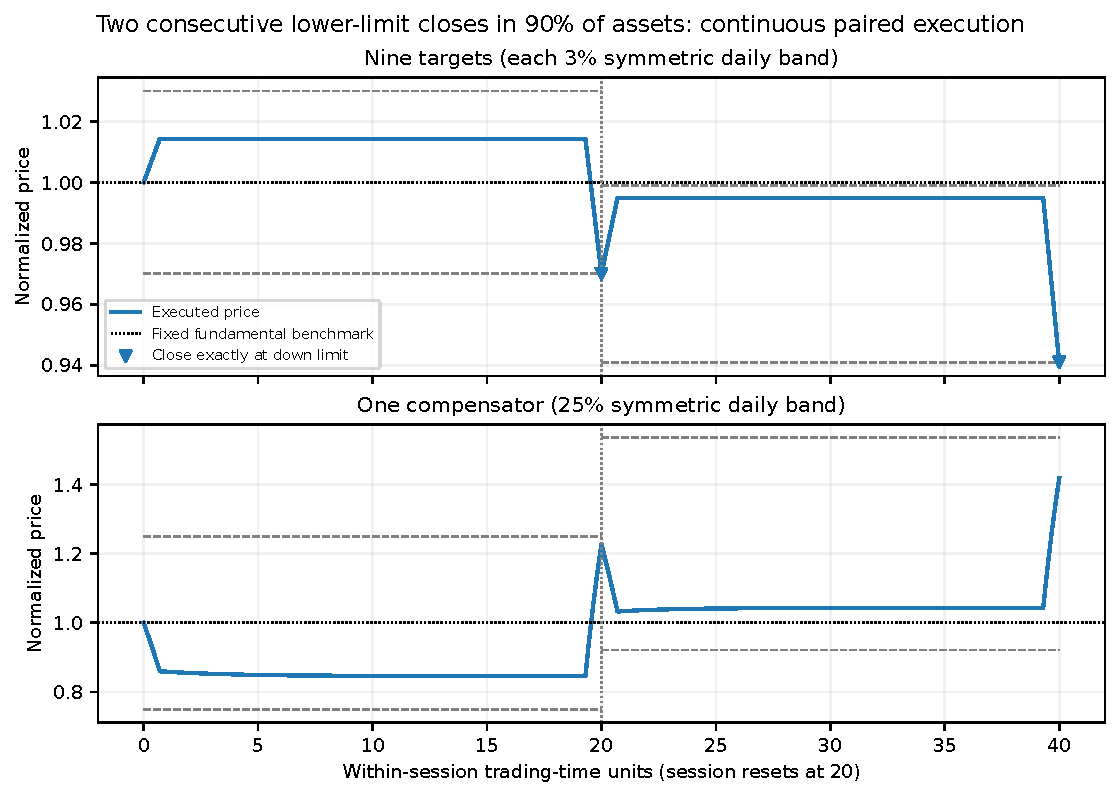
\includegraphics[width=.94\linewidth]{../../supplementary/figures/multiday_streak_witness.pdf}
\caption{\textbf{ローリング日次値幅下の一部資産の反復下限終値。} 同じ九対象資産が 3\%下限で二回引ける。第十の広い値幅の補償資産は自身の 25\%制限内にある。表示経路に瞬間取引はない。期間と値幅は指定モデル入力であり、観測値ではない。}\label{fig:streak-witness}
\end{figure}
\begin{figure}[tbp]\centering
 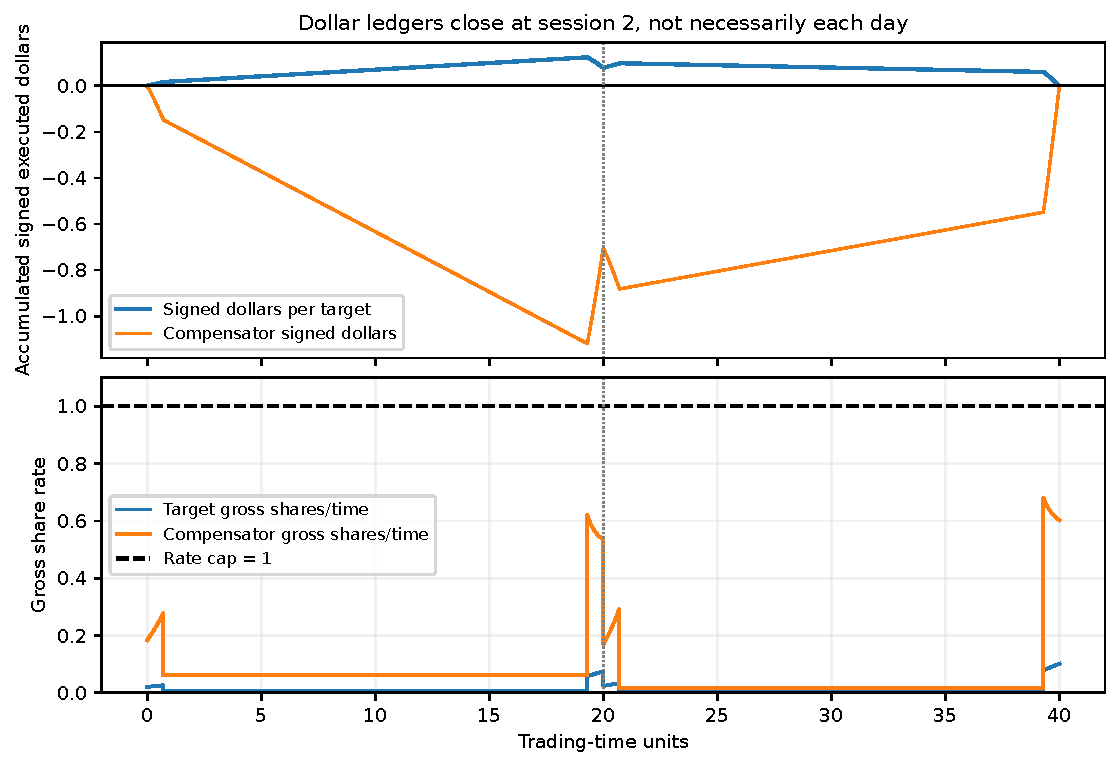
\includegraphics[width=.94\linewidth]{../../supplementary/figures/multiday_ledgers_and_rates.pdf}
\caption{\textbf{同じ二セッション構成例の取引元帳と総速度検査。} 第一セッションが対象の正の純売買代金フローを蓄積し、第二がこれを反転して、全資産の最終符号付き残高をゼロにする。総速度は株数速度上限未満である。売買代金均衡は満期だけでなく連続的に課す。}\label{fig:streak-ledger}
\end{figure}

本例は、取引者の実行誘因も、\emph{張り付いた}ストップ安注文板も証明しない。一方、ローリング値幅、有限株数執行速度、ファンダメンタルズのニュースショック不在、終端売買代金ゼロ条件は、広範な資産部分集合の\emph{複数回}の下限終値と両立しうることを数値的に示す。危機閾値には対象範囲条件だけで不十分である。この経路では$Q_{0.9}(T_2)=0.060918$だが平均損失制約が拘束的で$\Cris_{0.9}(T_2)=0.019932$となる（例えば$\delta=0.015$に到達する）。厳密な最小速度、最小売買代金、均衡発生を主張しない。



\section*{その他の診断図}
\begin{figure}[tbp]
\centering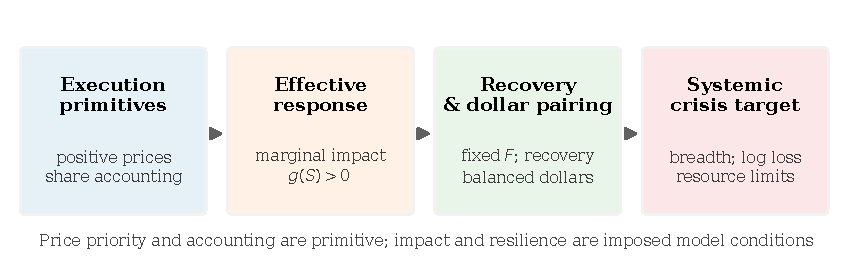
\includegraphics[width=.99\linewidth]{../../supplementary/figures/market_specification.pdf}
\caption{\textbf{明示的に定義した一つの理想市場。} 価格優先、符号付き株数会計、有効価格インパクト、回復力、売買代金ペア取引は異なる数学的役割を持つ。全定量図表は指定モデルの例示であり、稼働中注文板の観測ではない。}\label{fig:market}
\end{figure}
\begin{figure}[tbp]
\centering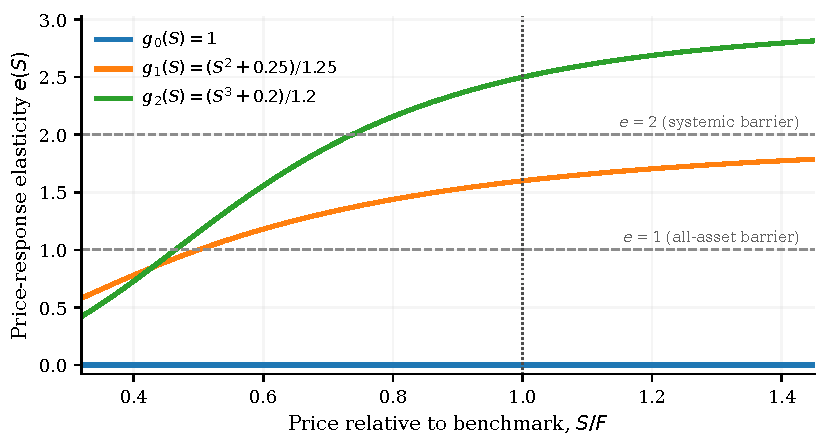
\includegraphics[width=.79\linewidth]{../../supplementary/figures/elasticity_examples.pdf}
\caption{\textbf{正で滑らかな三つの非べき乗インパクト関数の局所弾力性。} 縦点線は共通初期価格$S=F$である。主論文の大域的弾力性障壁定理は\emph{関連する到達可能価格領域}全体で弾力性不等式を要求する。$F$での値だけでは大域分類はできない。数式による例示であり、実証市場厚みではない。}\label{fig:elasticity}
\end{figure}
\begin{figure}[t]
\centering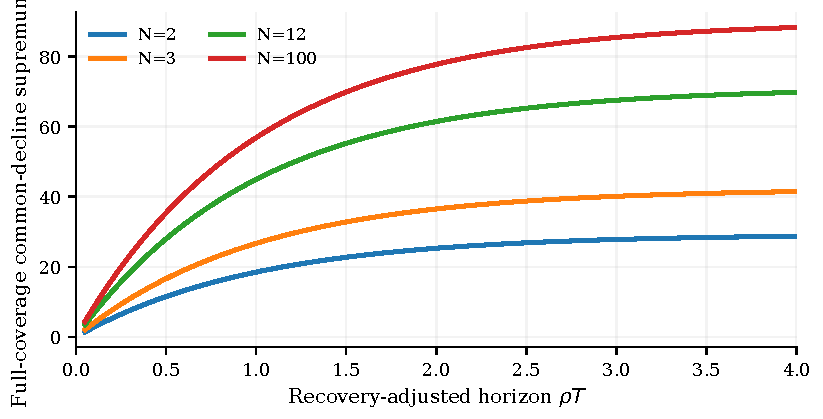
\includegraphics[width=.78\linewidth]{../../supplementary/figures/full_coverage_threshold.pdf}
\caption{\textbf{モデル固有の鋭い共通下落境界。} $g=\eta$、$k=N$では共通単純価格下落の上包絡線は$100(1-e^{-\delta_{\rm crit}})\%$である。厳密に小さい各対数損失閾値は有限予算で到達可能だが、境界自体は厳密正価格では達成されない。確率曲線ではない。}\label{fig:sharp}
\end{figure}
\begin{figure}[tbp]
\centering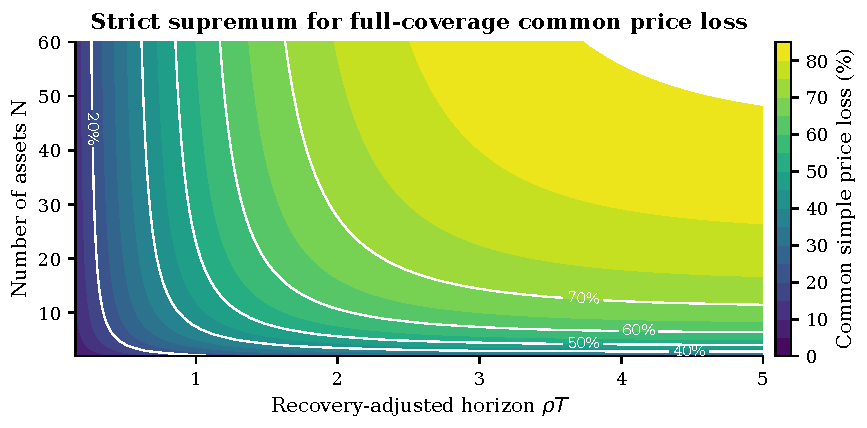
\includegraphics[width=.83\linewidth]{../../supplementary/figures/all_asset_boundary_heatmap.pdf}
\caption{\textbf{資産数と回復時間に対する全資産境界。} 色は$100(1-e^{-\delta_{\rm crit}(N,T)})$を示し、株当たり一定インパクトで個別終端売買代金がゼロの同時\emph{単純価格}損失の上限である。確率、観測ドローダウン、有限予算最適値を推論しない。}\label{fig:heatmap}
\end{figure}
\begin{figure}[tbp]
\centering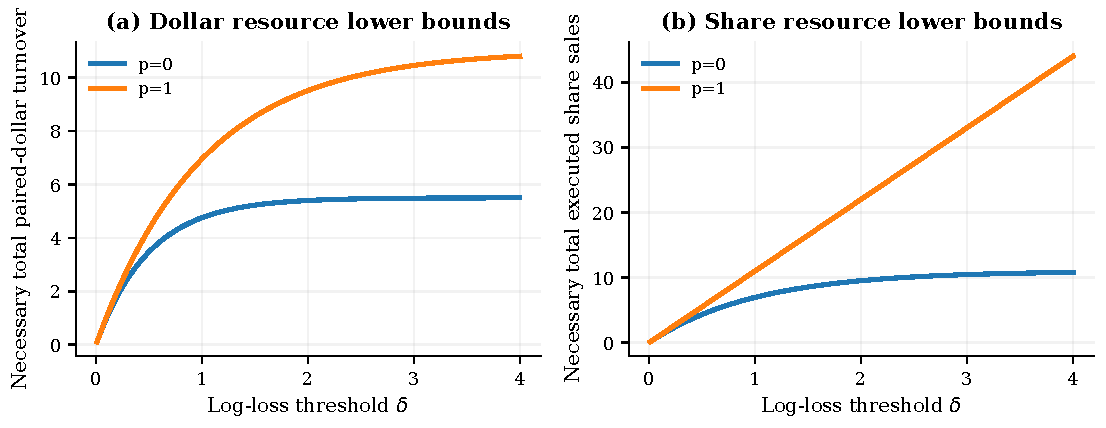
\includegraphics[width=.96\linewidth]{../../supplementary/figures/resource_lower_bounds.pdf}
\caption{\textbf{べき乗応答族による一般必要資源下限の例示。} $F=\eta=1$、$k=11$で、曲線は$k\int_{e^{-\delta}}^1 S/g(S)\dd S$（売買代金）と$k\int_{e^{-\delta}}^1 1/g(S)\dd S$（株数）を$p=0,1$について評価する。最適執行費用\emph{ではなく}、到達可能性を示さない。}\label{fig:resource}
\end{figure}
\begin{figure}[tbp]
\centering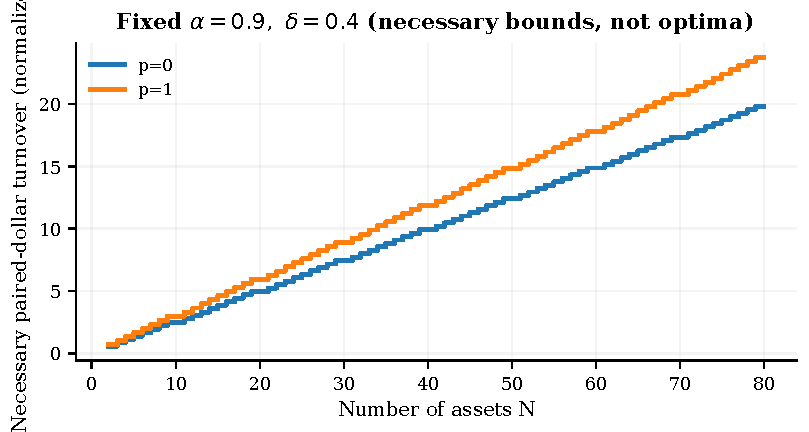
\includegraphics[width=.78\linewidth]{../../supplementary/figures/resource_scaling_N.pdf}
\caption{\textbf{必要売買代金資源下界の資産数依存。} 資産別基準価格・応答パラメータを複製し、$\alpha=0.9$、$\delta=0.4$を固定し、資産数$N$を増やす。段差は離散対象数$\lceil\alpha N\rceil$から生じる。実際の株価指数の時価総額調整予測ではない。}\label{fig:nscale}
\end{figure}
\begin{figure}[tbp]\centering
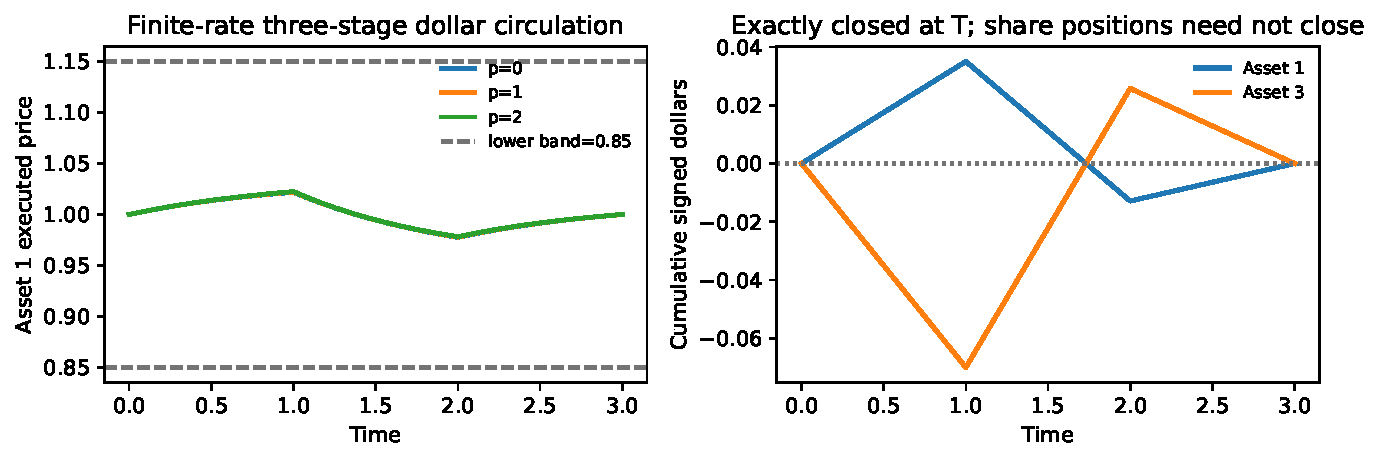
\includegraphics[width=.97\linewidth]{../../supplementary/figures/bounded_rate_continuous_path.pdf}
\caption{\textbf{新しい有界速度・終端売買代金ゼロ経路（パルス近似ではない）。} $N=3$、$T=3$、$a=.035$、$F=\rho=\eta=1$、$u=(1,1,-2)$で、$p=0,1,2$の価格軌道は同じ絶対連続売買代金速度信号を共有する。右図は厳密にゼロで閉じる元帳である。資産別総株数速度ピークは$0.15$未満で、全価格は$\pm15\%$値幅内にある。}\label{fig:continuous}
\end{figure}
\begin{figure}[tbp]\centering
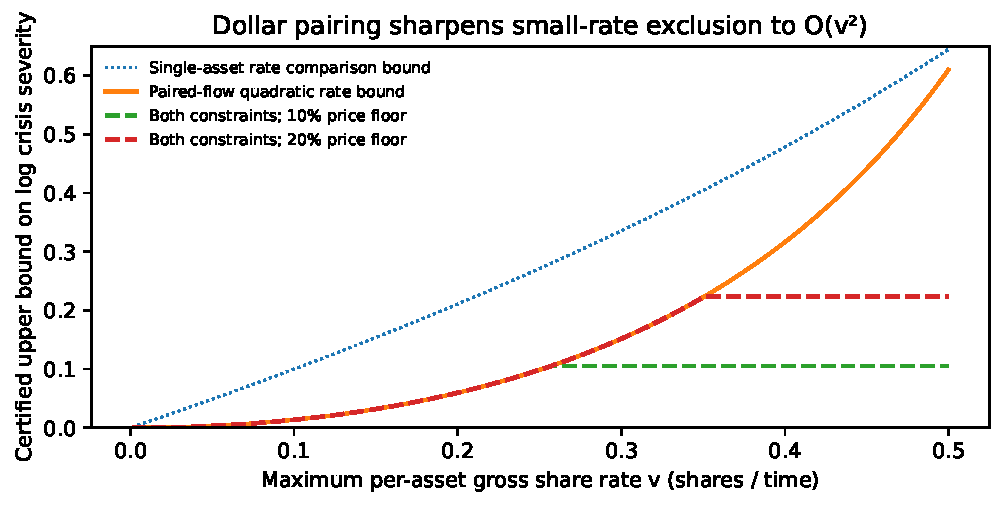
\includegraphics[width=.78\linewidth]{../../supplementary/figures/rate_and_price_limit_bounds.pdf}
\caption{\textbf{厳密到達最大値ではなく排除証明。} $g=\eta=F=\rho=1$、$T=3$で、ペアフロー二次評価は小速度の単一価格比較を改善し、単一セッション下限値幅は追加絶対上限を与える。いずれも最適危機制御や観測市場頻度を報告しない。}\label{fig:regulation}
\end{figure}
\begin{figure}[tbp]\centering
 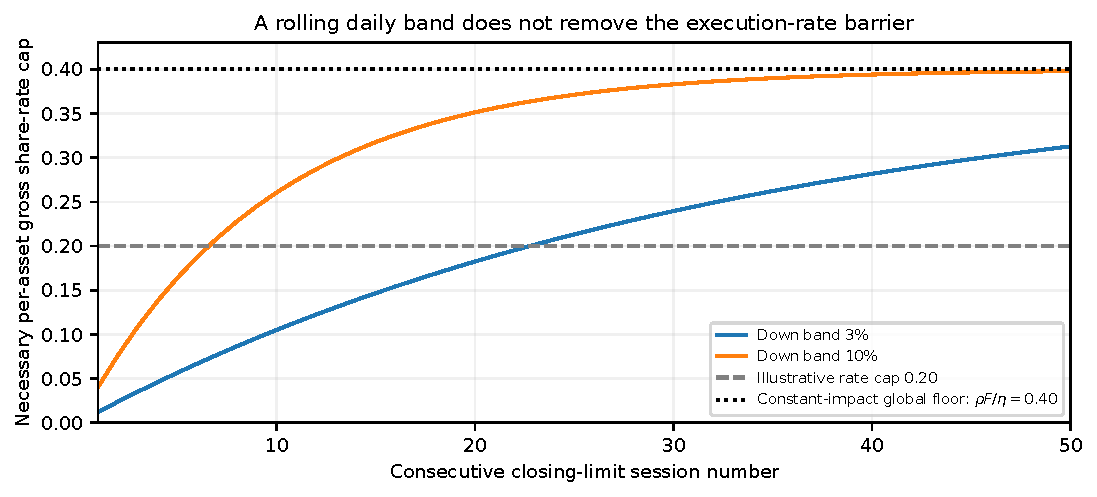
\includegraphics[width=.88\linewidth]{../../supplementary/figures/multiday_rate_frontier.pdf}
\caption{\textbf{反復下限終値に必要な総株数速度下限。} 主論文のスカラー一定インパクト比較モデルの必要速度公式を、$F=\eta=1$、$\rho=0.4$、$\tau=20$で示す。資産別\emph{必要}速度であり、ペア執行、利用可能在庫、補償資産自身の日次値幅により実際の市場閾値は高くなりうる。}\label{fig:streak-rate}
\end{figure}
\begin{figure}[tbp]\centering
 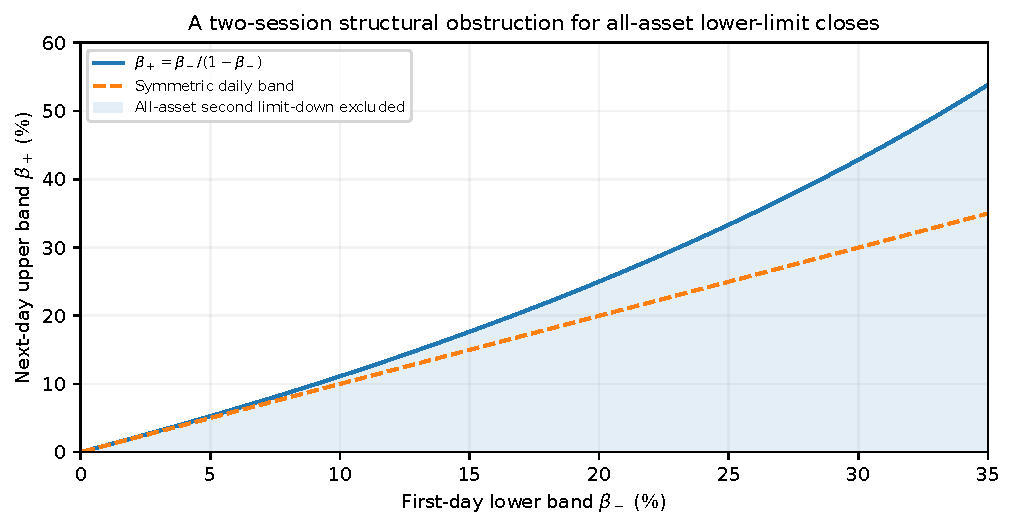
\includegraphics[width=.73\linewidth]{../../supplementary/figures/multiday_fullbreadth_obstruction.pdf}
\caption{\textbf{二回目の全資産下限終値が排除されるパラメータ領域。} 曲線下は$(1+\beta_+)(1-\beta_-)\le1$を満たす。対称比例値幅は領域の厳密内部にある。条件付き不変領域結果であり、取引所全体の注文列モデルではない。}\label{fig:streak-full-obstruction}
\end{figure}
\begin{figure}[tbp]\centering
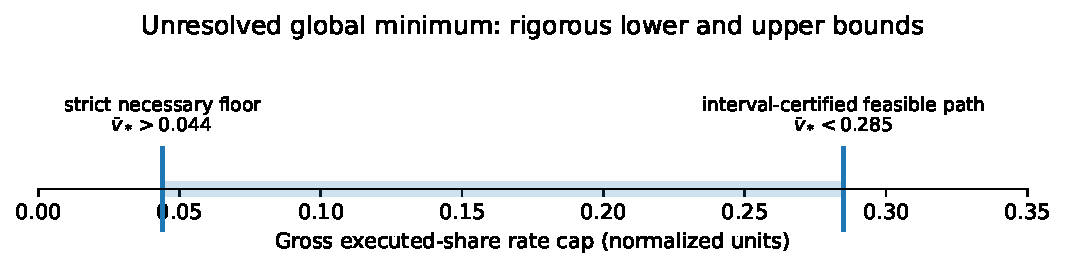
\includegraphics[width=.80\linewidth]{../../supplementary/figures/v7_minimum_rate_bracket.pdf}
\caption{\textbf{最適化済み事項と未最適化事項。} 既存二次システミック上界の厳密速度下限と認証済み実行可能経路が、未知の大域最小$\bar v_*$を挟む。区間は論理的許容性の範囲であり、統計的信頼区間ではない。}\label{fig:v7bracket}
\end{figure}
\begin{figure}[tbp]\centering
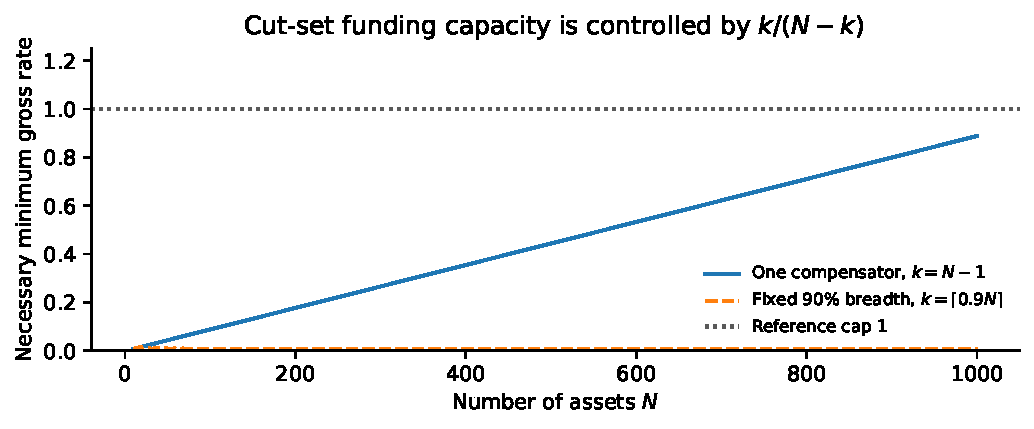
\includegraphics[width=.80\linewidth]{../../supplementary/figures/v7_cut_capacity_N.pdf}
\caption{\textbf{下落多数派の拡大に伴い増す資金受入容量制約。} 単一資産が拡大多数派の純ペア売買代金を吸収すると、主論文の第二日必要速度は$k/(N-k)$に比例して増す。図示した全$N$で実行可能市場が存在するとは証明しない。}\label{fig:v7cutN}
\end{figure}
\begin{figure}[tbp]\centering
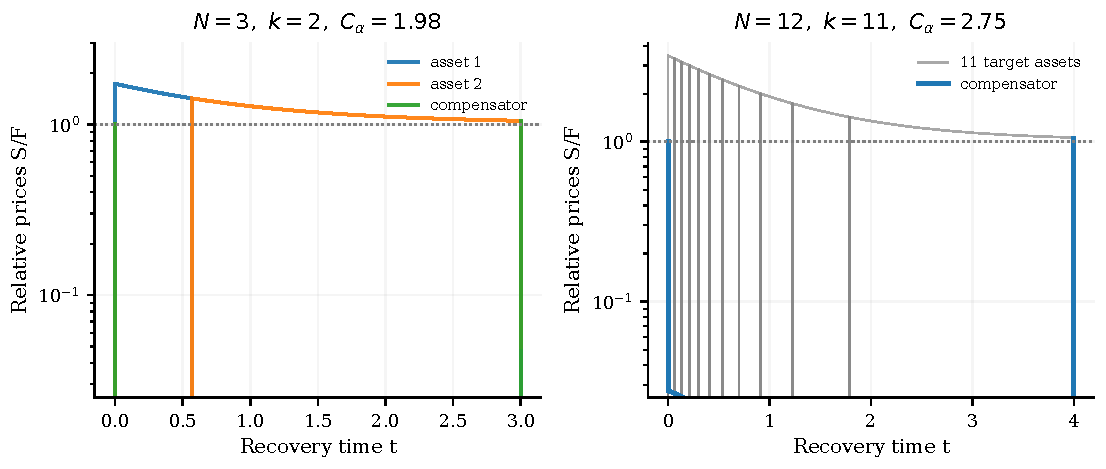
\includegraphics[width=.98\linewidth]{../../supplementary/figures/closed_flow_price_paths.pdf}
\caption{\textbf{終端売買代金ゼロの構成価格経路。} $N=3$、$N=12$で、一補償資産は初期値を上回り、残る$N-1$価格は共通目標対数損失$L=3$だけ下落する。対数縦軸でゼロ近傍価格を可視化する。折れと跳躍は許容制御パルスであり、模擬取引所イベントではない。}\label{fig:paths}
\end{figure}
\begin{figure}[tbp]\centering
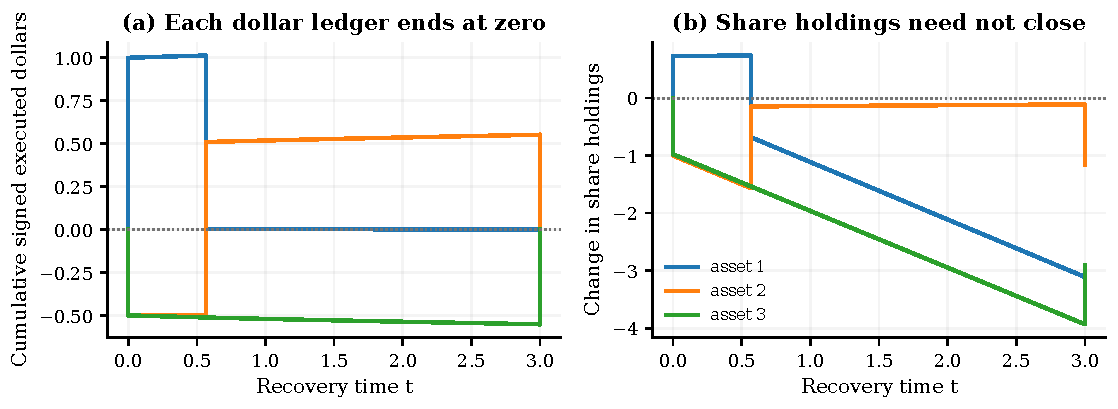
\includegraphics[width=.97\linewidth]{../../supplementary/figures/dollar_vs_share_closure.pdf}
\caption{\textbf{純売買代金は純株数ではない。} 別の$N=3$、$k=2$、$T=3$、$L=5$構成例は全資産で$X_i(T)=0$（左）を満たすが、純株数ポジションは一般にゼロと異なる（右）。初期在庫は総売却を賄う必要があり、取引ゼロ条件だけでは供給されない。}\label{fig:closure}
\end{figure}
\begin{figure}[tbp]\centering
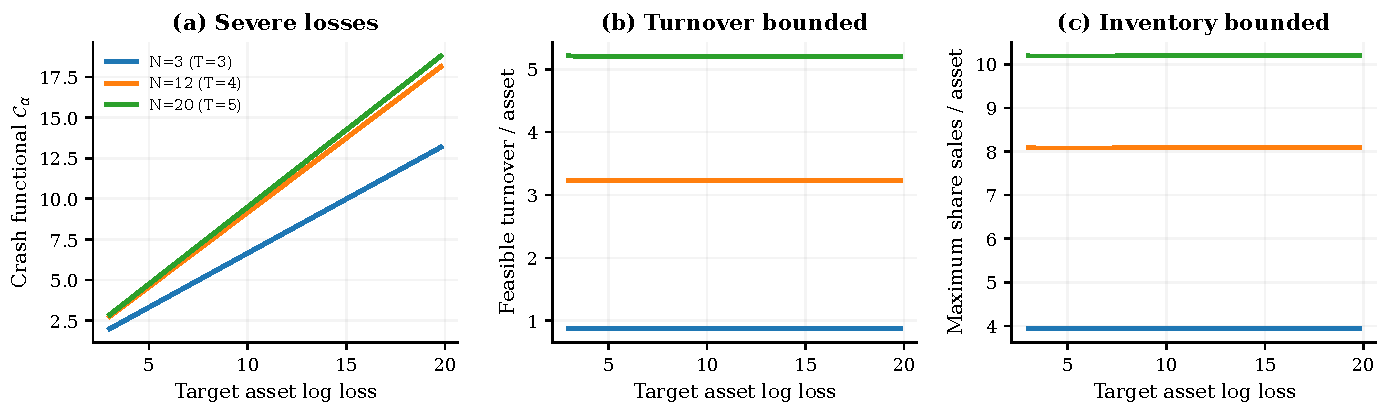
\includegraphics[width=.99\linewidth]{../../supplementary/figures/finite_resources_severe_crashes.pdf}
\caption{\textbf{有界な\emph{実行可能}資源の下で増す危機深度。} 選んだ$N=3,12,20$の構成族は$k=N-1$と期間$T=3,4,5$をそれぞれ用いる。終端目標価格対数損失が増すと$\mathcal C_\alpha$は増加する（左）が、経路の資産当たり売買代金（中央）と最大累積売却株数（右）は有界である。異なる期間・価格はモデル選択であり、市場間較正や最適値ではない。}\label{fig:finite}
\end{figure}
\begin{figure}[tbp]\centering
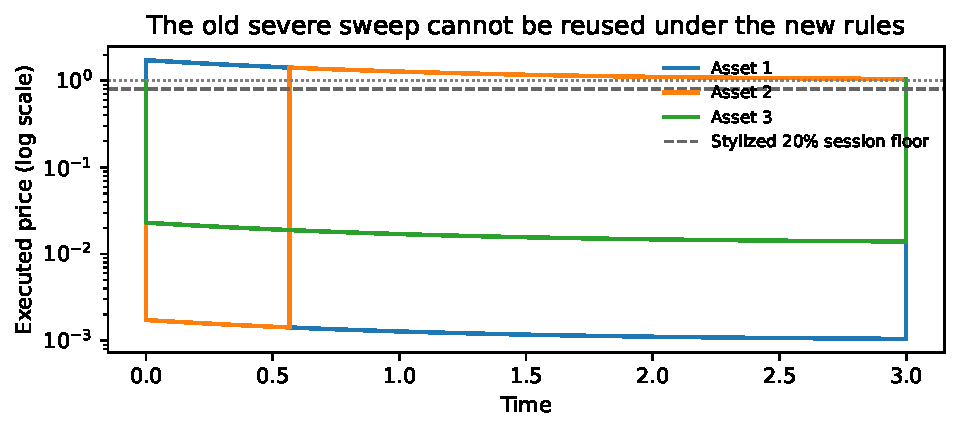
\includegraphics[width=.75\linewidth]{../../supplementary/figures/old_pulse_path_fails_limits.pdf}
\caption{\textbf{新執行制約による以前の深刻損失経路の診断的棄却。} 無制約モデルの$N=3$、$p=0$の深刻損失・終端売買代金ゼロ構成例は、仮想一セッション 20\%下限を越え、非ゼロ瞬間パルスを含む。ゆえに厳密ゼロ元帳は、有限総速度や値幅プロトコル下の到達可能性を認証\emph{しない}。}\label{fig:oldrejected}
\end{figure}\end{document}
